\chapter{Discrete Event Systems and Asset Allocation}\label{chpt:ED}
From this chapter on, we will adopt a different approach to the asset allocation problem: time will no longer be the driver of portfolio rebalancing but instead portfolio weights  will be updated whenever a predefined \textbf{event} occurs. This new point of view stems from the fact that when developing the stochastic reachability approach in Chapter \ref{chpt:Model_Description}, we let the system dynamics be indexed by an independent variable $k \in \mathbb{N}$ which we interpreted as discrete time but, as a matter of fact, the theory did not rely on this particular interpretation. This gives us the freedom to think of $k$ as an abstract index (for instance it could be an event counter). This observation is the basis for embedding the asset allocation problem in a \gls{DES} environment. 

In this chapter we will present the basics of \gls{DES} modeling (Section \ref{sec:Introduction_to_DES}) which are essential for discussing the \gls{ED} approach to asset allocation (Section \ref{sec:EventDrivenAA}). As far as the \gls{DES} is concerned, the main reference is the rich monograph \cite{cassandras2009}, whereas the \gls{ED} asset allocation model is taken from \cite{specchio2011}.

\section{Introduction to DES }\label{sec:Introduction_to_DES}
From a Control System point of view, the dynamical system introduced in (\ref{eq:state_equation}) can be classified as \textit{continuous-state} (the state space $\mathcal{X}$ is a proper subset of $\mathbb{R}$) and \textit{discrete-time} ($k \in \mathbb{N}$). Informally, if the state space is a discrete set and state transitions are observed whenever an "event" occurs we will talk about Discrete Event Systems. Systems considered so far are time-driven, in that we could imagine the systems being synchronized to a clock and at every clock tick an event $e$ is drawn from an event space $E$ causing the state to change. However, we could think of a different mechanism governing the state transition: at various time instants (not necessarily known in advanced), some event $e \in E$ occurs, making the state change.
The following example will hopefully clarify the difference between \gls{TD} and \gls{ED} systems. Imagine a particle bound to move on a plane; at every tick of a clock an event is drawn and the particle is allowed to move by a unit step in direction North, South, East or West. In this case we have a \gls{TD} system whose events are $e_1= \text{"one step North"}$, $e_2= \text{"one step South"}$ and so on. On the other hand, suppose there are four players, each of them capable of making the particle move in his direction by issuing a signal. A player issues a signal at random times. The resulting system is \gls{ED} since it is not synchronized to any clock and state transitions are caused by event like $e_k=$"player 1 issued a signal". The formal definition of a \gls{DES} reads as follows
\begin{definition}[Discrete Event System]
	A \textbf{Discrete Event System} is a \textit{discrete-state}, \textit{event-driven} system, that is, its state evolution depends entirely on the occurrence of asynchronous discrete events over time.
\end{definition} 


A \gls{DES} can be studied from three different levels of abstraction. We will present them in increasing order of complexity
\begin{enumerate}
	\item \textit{untimed}: the interest is on the sequences of events that the system could execute, without any time information. For instance, an untimed sequence could be
	\[e_1, e_2, e_3, e_4, e_5, e_6 \]
	\item \textit{timed}: in this representation each possible event sequence is coupled with time information, that is, not only the order of occurrence is given but also the exact time instant an event occurred. For example, in the \textit{timed} setting, the following could be a system sample path
	\[(e_1,t_1), (e_2,t_2), \ldots, (e_6,t_6) \]
	
	
	\item \textit{stochastic timed}: it is the most detailed description of a \gls{DES} since it contains event information on all possible orderings, time information about the exact instant at which the event occurs and also statistical information about successive occurrences.
\end{enumerate}
As our modeling purposes required the stochastic timed level of abstraction, we now give the definition of a \textit{Stochastic Clock Structure} which is the tool used to include time and statistical information to a sequence of events.
\begin{definition}[Stochastic Clock Structure]
	The \textbf{Stochastic Clock Structure} associated with an event set $E$ is a set of CDFs
	\[ \bm{G} = \{G_i \colon i \in E \}   \]
	characterizing the stochastic clock sequences
	\[ \bm{V}_{i} = \{V_{i,1},V_{i,2},\ldots \} \qquad i \in E \]
	where $V_{i,k}$ is a random variable indicating the k-th occurrence time of event $e_i$.
\end{definition}
\begin{remark}
	Sometimes, instead of modeling the exact time when an event occurs (as in the definition above), it is more convenient to model the elapsed time between two events, the so-colled \textbf{interevents time}. In this case we will write the Stochastic Clock Sequence in the following way \[ \bm{T}_{i} = \{T_{i,1},T_{i,2},\ldots \} \qquad i \in E. \]
\end{remark}
If a deterministic clock sequence  $\bm{v}_i = \{v_{i,1}, v_{i,2},\ldots\}$ is given for each event in $E$, we will talk about a \textit{Clock Structure} (this is the case in the \textit{timed} case). The evolution of a \gls{DES} needs to be described by a state equation of the form
\begin{equation}\label{eq:untimed_dynamics}
x_{k+1} = f(x_k,e_{k+1}) \qquad k \in \mathbb{N}
\end{equation}
where $x_k$ is the current state and $x_{k+1}$ the state once the event $e_{k+1}$ has occurred. The above recursive equation is the event-driven equivalent of Equation (\ref{eq:state_equation}). However, Equation (\ref{eq:untimed_dynamics}) describes only the untimed dynamics, that is no time information is included. Conversely, in asset allocation applications, we are interested also in \textit{when} an event occurs. For this reason, after introducing a Clock Structure $\bm{v} = \{v_i \colon i \in E\}$ associated with a finite event set $E = \{e_1,\ldots,e_n\}$, we seek a relationship of the form \[ e_{k+1} = h(x_k,\bm{v}_1,\ldots,\bm{v}_n)\] so that we could replace (\ref{eq:untimed_dynamics}) with
\begin{equation}\label{eq:timed_dynamics}
\begin{cases}
x_{k+1} & = f(x_k,e_{k+1})\\
e_{k+1} & = h(x_k,\bm{v}_1,\ldots,\bm{v}_n).
\end{cases}
\end{equation}
Equations (\ref{eq:timed_dynamics}) capture the \textit{timed} dynamics of a \gls{DES}.

As it was mentioned earlier, the \text{Stochastic timed} behavior is what interests us; therefore, we conclude this section by giving the definition of a Stochastic Timed Automaton which is the theoretical modeling structure of a \gls{DES} (see \cite{cassandras2009} for a more detailed treatment)
\begin{definition}[Stochastic Timed Automaton]
	A \textbf{Stochastic Timed Automaton} is a six-tuple \[ (\mathcal{E},\mathcal{X},\Gamma,p,p_0,\bm{G})\]
	where 
	\begin{description}
		\item[$\mathcal{E}$] is a countable event set
		\item[$\mathcal{X}$] is a countable state space
		\item[$\Gamma(x)$] is the set of feasible events, defined $\forall x \in \mathcal{X}$
		\item[$p(x';x,e')$] is the transition probability from state $x$ to state $x'$ given the occurrence of event $e'$
		\item[$p_0(x)$] is the pmf of the initial state $X_0$ (which is a random variable)
		\item[$\bm{G}=\{\bm{T}_i \colon i \in \mathcal{E}\}$] is a Stochastic Clock Time of interevent times.
	\end{description}
\end{definition}
A Stochastic Timed Automaton, together with the dynamics in Equation (\ref{eq:timed_dynamics}) (where the Clock Structure $\bm{v}$ is replaced by a Stochastic one $\bm{V}$) give the most complete description of a \gls{DES}. We now move to the asset allocation application.
\section{Event-Driven Asset Allocation}\label{sec:EventDrivenAA}
In this section we present the first event-driven model having in mind the objective to invest in the derivative market. In fact, we will consider a market consisting of a \textbf{risky asset} (a future index) and a \textbf{risk-free asset} (a bank account). The event-driven approach aims at modeling the industrial practice of rebalancing the portfolio weights whenever an "event" occurs. In the following, we suppose that an event has occurred every time the absolute value of the risky return hits a threshold (e.g. 7\%). This policy could be beneficial in different aspects:
\begin{enumerate}
	\item in low-volatile markets, when the risky asset price is quite steady, portfolio weights need not to be updated at predefined time instants but only when the market conditions have significantly changed. This cuts down on transaction costs.
	\item in high-volatile markets, when the risky asset price repetitively increases or plummets in a short period of time (shorter than the rebalancing frequency), the event-driven policy can swiftly intervene by changing the portfolio exposure without having to wait the rebalancing time (when the loss could already be substantial).
\end{enumerate}
The main goal of this section is first to derive a proper event-driven dynamics of the portfolio value and then find its density function which will be plugged in the ODAA algorithm.
Let us now start off by investigating both the time-driven dynamics (which will allow us to estimate how long the investment is going to last) and the event-driven dynamics.
\subsection{Time-driven dynamics}
A portfolio rebalancing is performed every time the absolute value of the risky asset cumulative return, starting from an initial baseline, hits a threshold. Let $J$ be this threshold. We suppose the following time-driven discrete dynamics for the risky asset
\begin{equation}\label{eq:time_driven_dynamics}
S_{k+1} = S_k(1 + J N^{\Delta t}_{k+1}) \qquad k \in \mathbb{N}.
\end{equation}
The random variable $N^{\Delta t}_{k+1}$ (which is the k+1-th element of a sequence of iid random variables) takes values in the discrete set $\{1,0,-1\}$ and indicates whether the discrete price process has a positive, negative or null jump at the end of a time interval of length $\Delta t$. If it takes the value 1, the discrete price process $\{S_k\}$ experiences a positive jump at the end of time period $[t_k,t_{k+1}]$, if the value is -1 then the jump is negative and if the value is 0, the process has no jumps in this time interval. This is the same as saying that when the random variable takes the value 1 then the risky asset cumulative return is greater than J, when the value is -1 then the cumulative return is smaller than -J and when the value is 0, than it belongs to the interval $[-J,J]$. The superscript $\Delta t$ indicates the length of the interval $[t_k,t_{k+1}]$. The next step is to find a proper distribution for $N^{\Delta t}_{k+1}$.
Let the probability mass function (pmf) of this random variable  have the following form
\begin{equation}\label{eq:pmf_time_driven}
f_{N^{\Delta t}_{k+1}}(y) = 
\begin{cases}
 \exp\{-\lambda \Delta t\} & \text{if } y = 0 \\
 \big(1-\exp\{-\lambda \Delta t\}\big)p & \text{if } y = 1 \\
 \big(1-\exp\{-\lambda \Delta t\}\big)(1-p) & \text{if } y = -1
\end{cases}
\end{equation}
where $\lambda \in \mathbb{R}^{+}$ and $p \in [0,1]$. This functional form is particularly convenient since it implies an exponential distribution for the interevent times (also called \textbf{holding times} in a financial context). This fact is synthesized in the following proposition
\begin{proposition}\label{prop:tau_distribution}
	Given the time-driven dynamics of the risky asset in (\ref{eq:time_driven_dynamics}) and the pmf (\ref{eq:pmf_time_driven}) of random variable $N^{\Delta t}_{k+1}$, let $\tau_{k+1}$ be the random variable indicating the holding time between the $k$-th and the $(k+1)$-event.
	Then $\tau_{k+1} \sim \text{exp}(\lambda)$
\end{proposition}
\begin{proof}
	Let $t_k$ be a realization of the random variable $T_k$, which is an element of a Stochastic Clock Sequence and therefore indicates when the $k$-th event occurs. From the definition of a Stochastic Clock Structure we have
	\[
	G_{k+1}(t)= \mathbb{P}\big(\tau_{k+1}\leq t\big) = 1 - \mathbb{P}\big(\tau_{k+1}> t\big)
	\]
	but 
	\begin{align*}
	\mathbb{P}\big(\tau_{k+1}>t \lvert T_k = t_k\big) &= \mathbb{P}\big(N^{(t_k+t)-t_k}_{k+1}=0\big)\\
	& =\mathbb{P}\big(N^{t}_{k+1}=0\big)  \\
	& = \exp\{-\lambda t \}
	\end{align*}
	therefore $\mathbb{P}\big(\tau_{k+1}>t \lvert T_k = t_k\big)$ is independent from $t_k$. Hence 
	\[
	\mathbb{P}\big(\tau_{k+1}>t \lvert T_k = t_k\big) = \mathbb{P}\big(\tau_{k+1}> t\big) = \exp\{-\lambda t \} 
	\]
	which implies $G_{k+1}(t)=1-\exp\{-\lambda t \}$. Since this is the cdf of an exponential random variable, we have the result.
\end{proof}
\begin{remark}
	Given that $\mathbb{E}[\tau_{k+1}]=\frac{1}{\lambda}$, the parameter $\lambda$ acquires the meaning of speed of the discrete dynamics. The larger it is, the more frequent portfolio rebalancings are.
\end{remark}
\subsection{Event-driven dynamics}
Dynamics (\ref{eq:time_driven_dynamics}) is still time-driven since the independent variable $k \in \mathbb{N}$ represents discrete time. Instead, in the event-driven framework, we let $k$ indicate the number of events (portfolio rebalancings/trades). For example, $S_{k+1}$ is the risky asset price after the k+1-th portfolio rebalancing is performed. The event-driven dynamics of the risky asset reads as follows
\begin{equation}\label{eq:event_driven_dynamics}
S_{k+1} = S_{k}(1+J \widetilde{N}_{k+1}) \qquad k \in \mathbb{N}
\end{equation}
where $\widetilde{N}_{k+1}$ is distributed according to 
\begin{equation}\label{eq:pmf_event_driven}
f_{\widetilde{N}_{k+1}}(y)  = 
\begin{cases}
p & \text{if } y = 1 \\
1-p & \text{if } y = -1
\end{cases}
\end{equation}
Let us understand how the pmf (\ref{eq:pmf_event_driven}) follows from (\ref{eq:pmf_time_driven}). First of all, the random variable $\widetilde{N}_{k+1}$ is Bernoullian. In fact, it models whether the jump is positive or negative. Therefore we are left to compute the probability of the jump to be positive (the parameter $q$ of the Bernoulli distribution). By applying the Bayes Theorem, the Law of Total Probability in the continuous case and the fact that $\tau_{k+1}$ is exponential with parameter $\lambda$, we obtain
\begin{align*}
q &= \mathbb{P}\big(\widetilde{N}_{k+1} = 1\big) = \mathbb{P}\big(N_{k+1}^{\tau_{k+1}}=1\lvert(N_{k+1}^{\tau_{k+1}}=0)^C\big)\\[1.5ex]
& = \frac{\mathbb{P}\big(N_{k+1}^{\tau_{k+1}}=1,(N_{k+1}^{\tau_{k+1}}=0)^C\big)}{\mathbb{P}\big((N_{k+1}^{\tau_{k+1}}=0)^C\big)}\\[1ex]
&=\frac{\mathbb{P}\big(N_{k+1}^{\tau_{k+1}}=1\big)}{1-\mathbb{P}\big(N_{k+1}^{\tau_{k+1}}=0\big)}\\[1.5ex]
& = \frac{\int_{0}^{\infty}\mathbb{P}\big(N_{k+1}^{\tau_{k+1}} = 1\lvert\tau_{k+1}=t\big)f_{\tau_{k+1}}(t)\mathrm{d}t}{1-\int_{0}^{\infty}\mathbb{P}\big(N_{k+1}^{\tau_{k+1}} = 0\lvert\tau_{k+1}=t\big)f_{\tau_{k+1}}(t)\mathrm{d}t}\\[1.5ex]
& = \frac{\int_{0}^{\infty}(1-e^{-\lambda t})p\lambda e^{-\lambda t} \mathrm{d}t  }{1-\int_{0}^{\infty}e^{-\lambda t}\lambda e^{-\lambda t}\mathrm{d}t } \\[1.5ex]
& = p
\end{align*}
Parameter $p$ governs the trend of the discrete price process. The greater $p$, the more likely it is to have positive jumps.

\subsection{Portfolio dynamics}
We recall that the portfolio we are considering consists of a risky and a risk-free asset. The event-driven dynamics of the former has been given in (\ref{eq:event_driven_dynamics}). In this section the event-driven dynamics of portfolio value will be derived. For the sake of simplicity, we assume that the risk-free asset evolves in a deterministic way with interest rate $r$ (continuously compounded). Throughout this section, let us fix two time instants, $t_k$ and $t_{k+1}$, which are realizations of random variables $T_k$ and $T_{k+1}$. These random variables indicate the time when the k-th and k+1-th trade takes place (or, in other words, when the k-th and k+1-th event occur).

In general, the event-driven portfolio dynamics is
\begin{equation}\label{eq:general_ptf_dynamics}
x_{k+1} = x_k(1+u_{k}^C w_{k+1}^{C} + u_{k}^S w_{k+1}^S) \qquad k \in \mathbb{N}
\end{equation}
where $u_{k}^C$, $u_{k}^S$ are the portfolio weights of the risk-free and risky asset respectively, $w_{k+1}^{C}$ and $w_{k+1}^S$ their return over the period $[t_k,t_{k+1}]$. It is important to remark that the length of the time interval $[t_k,t_{k+1}]$ is not deterministic, but it is a random variable exponentially distributed (see Proposition \ref{prop:tau_distribution}), denoted by $\tau_{k+1}$. Consequently, $w_{k+1}^{C}$ and $w_{k+1}^S$ are returns over a stochastic time period. From (\ref{eq:event_driven_dynamics}) we easily get
\begin{equation}\label{eq:risky_return}
w_{k+1}^S=J\widetilde{N}_{k+1}
\end{equation}
As far as the risk-free asset in concerned, denoting by $C_{k+1}$ its price after the k+1-th trade, we have

\begin{align}\label{eq:riskfree_return}
	\nonumber
	&C_{k+1} = C_k(1+w_{k+1}^{C})^{\tau_{k+1}} = C_k \exp\{r \tau_{k+1}\}\\
	& \implies \quad w_{k+1}^{C} = \exp\{r \tau_{k+1}\}-1
\end{align}
where $r$ is the deterministic interest rate of the risk-free asset, continuously compounded. By plugging (\ref{eq:risky_return}) and (\ref{eq:riskfree_return}) into (\ref{eq:general_ptf_dynamics}) the portfolio dynamics becomes
\begin{equation}\label{eq:ptf_dynamic_ED}
\boxed{x_{k+1}= x_k(\exp\{r\tau_{k+1}\} + u_{k}J\widetilde{N}_{k+1} ) } \qquad k \in \mathbb{N}
\end{equation}	
where we dropped the superscript $S$ from $u_{k}^S$ and set $u_k^C=1$. This reflexes what is usually done in the derivative trading practice, namely keeping a 100\% cash position plus a long or short exposure to the derivative. Consequently, the weight $u_{k}$ is allowed to take values in the compact set $[-1,1]$. 

\subsection{The density of $x_{k+1}$}
In order to apply the ODAA algorithm (see Theorem \ref{thm:rec_algo}), the explicit form of the density of the random variable $x_{k+1}$ is required. The result is given in the following proposition
\begin{proposition}\label{prop:density_portfolio_basic}
	The probability density function of random variable (\ref{eq:ptf_dynamic_ED}) is
	\begin{equation*}
	f_{x_{k+1}}(z)= 
	\begin{cases}
	0         & \text{if } z < x-\xi \\[1ex]  
	\frac{\lambda}{r x}(1-p)\big(\frac{z+\xi}{x}\big)^{-(\frac{\lambda+r}{r})} & \text{if } x-\xi \leq z < x+\xi \\[1ex]  
	\frac{\lambda}{r x}\big[(1-p)\big(\frac{z+\xi}{x}\big)^{-(\frac{\lambda+r}{r})} + p \big(\frac{z-\xi}{x}\big)^{-(\frac{\lambda+r}{r})}\big]   & \text{if } z \geq x+\xi
	\end{cases}
	\end{equation*}
	where $\xi=xJu_{k+1}$.
\end{proposition}
\begin{proof}
	Let $F_{\tau_{k+1}}(t)= (1-e^{-\lambda t})\mathbbm{1}_{[0,\infty)}(t)$ be the cdf of $\tau_{k+1}$. The first step consists in finding the cdf $F_Y$ of $Y=x\exp\{r \tau_{k+1}\}$. By simple calculations we obtain
	\[F_Y(y)=\Big(1-\Big(\frac{y}{x}\Big)^{-\frac{\lambda}{r}}\Big)\mathbbm{1}_{[x,\infty)}. \]
	Let us rewrite the portfolio value at the k+1-th trade in the following way \[ x_{k+1} = Y + xu_kJ\widetilde{N}_{k+1}=Y+\xi \widetilde{N}_{k+1} \]
	and by using the Law of Total Probability we have
	\begin{align*}
	F_{x_{k+1}}(z) & = \mathbb{P}\big(Y+\xi \widetilde{N}_{k+1}\leq z\big)\\[1.5ex]
	& = \mathbb{P}\big(Y+\xi \widetilde{N}_{k+1}\leq z\lvert \widetilde{N}_{k+1}=1\big)\mathbb{P}\big(\widetilde{N}_{k+1}=1\big)+\\
	&\qquad +\mathbb{P}\big(Y+\xi \widetilde{N}_{k+1}\leq z\lvert \widetilde{N}_{k+1}=-1\big)\mathbb{P}\big(\widetilde{N}_{k+1}=-1\big)\\[1.5ex]
	& = F_Y(z-\xi)p+F_Y(z+\xi)(1-p)\\[1.5ex]
	& = \Big\{1-\Big(\frac{z-\xi}{x}\Big)^{-\lambda/r} \Big\}\mathbbm{1}_{[x+\xi,\infty)}+
	\Big\{1-\Big(\frac{z+\xi}{x}\Big)^{-\lambda/r} \Big\}\mathbbm{1}_{[x-\xi,\infty)}
	\end{align*}
	Differentiating the cdf we have the result:
	\begin{align*}
	f_{x_{k+1}}(z) & = \frac{\mathrm{d}}{\mathrm{d}z}F_{x_{k+1}}(z)\\
	& = \frac{\lambda}{r x}\Big\{p\Big(\frac{z-\xi}{x}\Big)^{-\big(\frac{\lambda+r}{r}\big)}\mathbbm{1}_{[x+\xi,\infty)} + 
	(1-p)\Big(\frac{z+\xi}{x}\Big)^{-\big(\frac{\lambda+r}{r}\big)}\mathbbm{1}_{[x-\xi,\infty)}\Big\}
	\end{align*}
\end{proof}


\section{The calibration of $p$ and $\lambda$}
In this section we calibrate the parameters $p$ and $\lambda$ of the pmf (\ref{eq:pmf_time_driven}) to market data. We recall that parameter $p$ is responsible of the trend of process $\{S_k\}$ whereas $\lambda$ controls the jump frequency. The time series we are considering is the daily Future S\&P 500 from 22 January 2010 to 25 April 2016. In order to find estimates $\widehat{p}$ and $\widehat{\lambda}$ we need to extract a sample of realizations of random variable $N_{k+1}^{\Delta t}$ from the above time series. This could be accomplished by applying Algorithm \ref{algo:discrete_price_process} to the data. Indeed,  the algorithm outputs the discrete time series (reported in red in Figure \ref{fig:DiscreteDynamics}) and the logical sample $\bm{y}=\{y_1,\ldots,y_n\}$ (denoted by $\{d_{t_k}\}_{k=1,\ldots,n}$ in the algorithm).
\begin{algorithm}[H]
	\SetAlgoLined
	\KwIn{price time series $\{S_{t_k}\}_{k=0,\ldots,n}$, jump size $J$}
	\KwOut{discrete price time series $\{D_{t_k}\}_{k=0,\ldots,n}$, logical time series $\{d_{t_k}\}_{k=1,\ldots,n}$}
	initialization: $Baseline = S_{t_0}$, $D_{t_0}=S_{t_0}$\;
	
	\For{$i = 1,\ldots,n$}{
		$R = S_{t_i}/Baseline - 1$\;
		
		\eIf{$abs(R) > J$}
		{$Baseline = Baseline(1+sign(r)J)$\;
			
		 $D_{t_i} = Baseline$ \;
		 
		 $d_{t_i}= sign(r)$	
		}{ 
		$D_{t_i} = D_{t_{i-1}}$ \;
		
		$d_{t_i}= 0$	
		}	
}
\caption{Discrete price and logical time series}
\label{algo:discrete_price_process}
\end{algorithm}
\begin{figure}
	\centering
	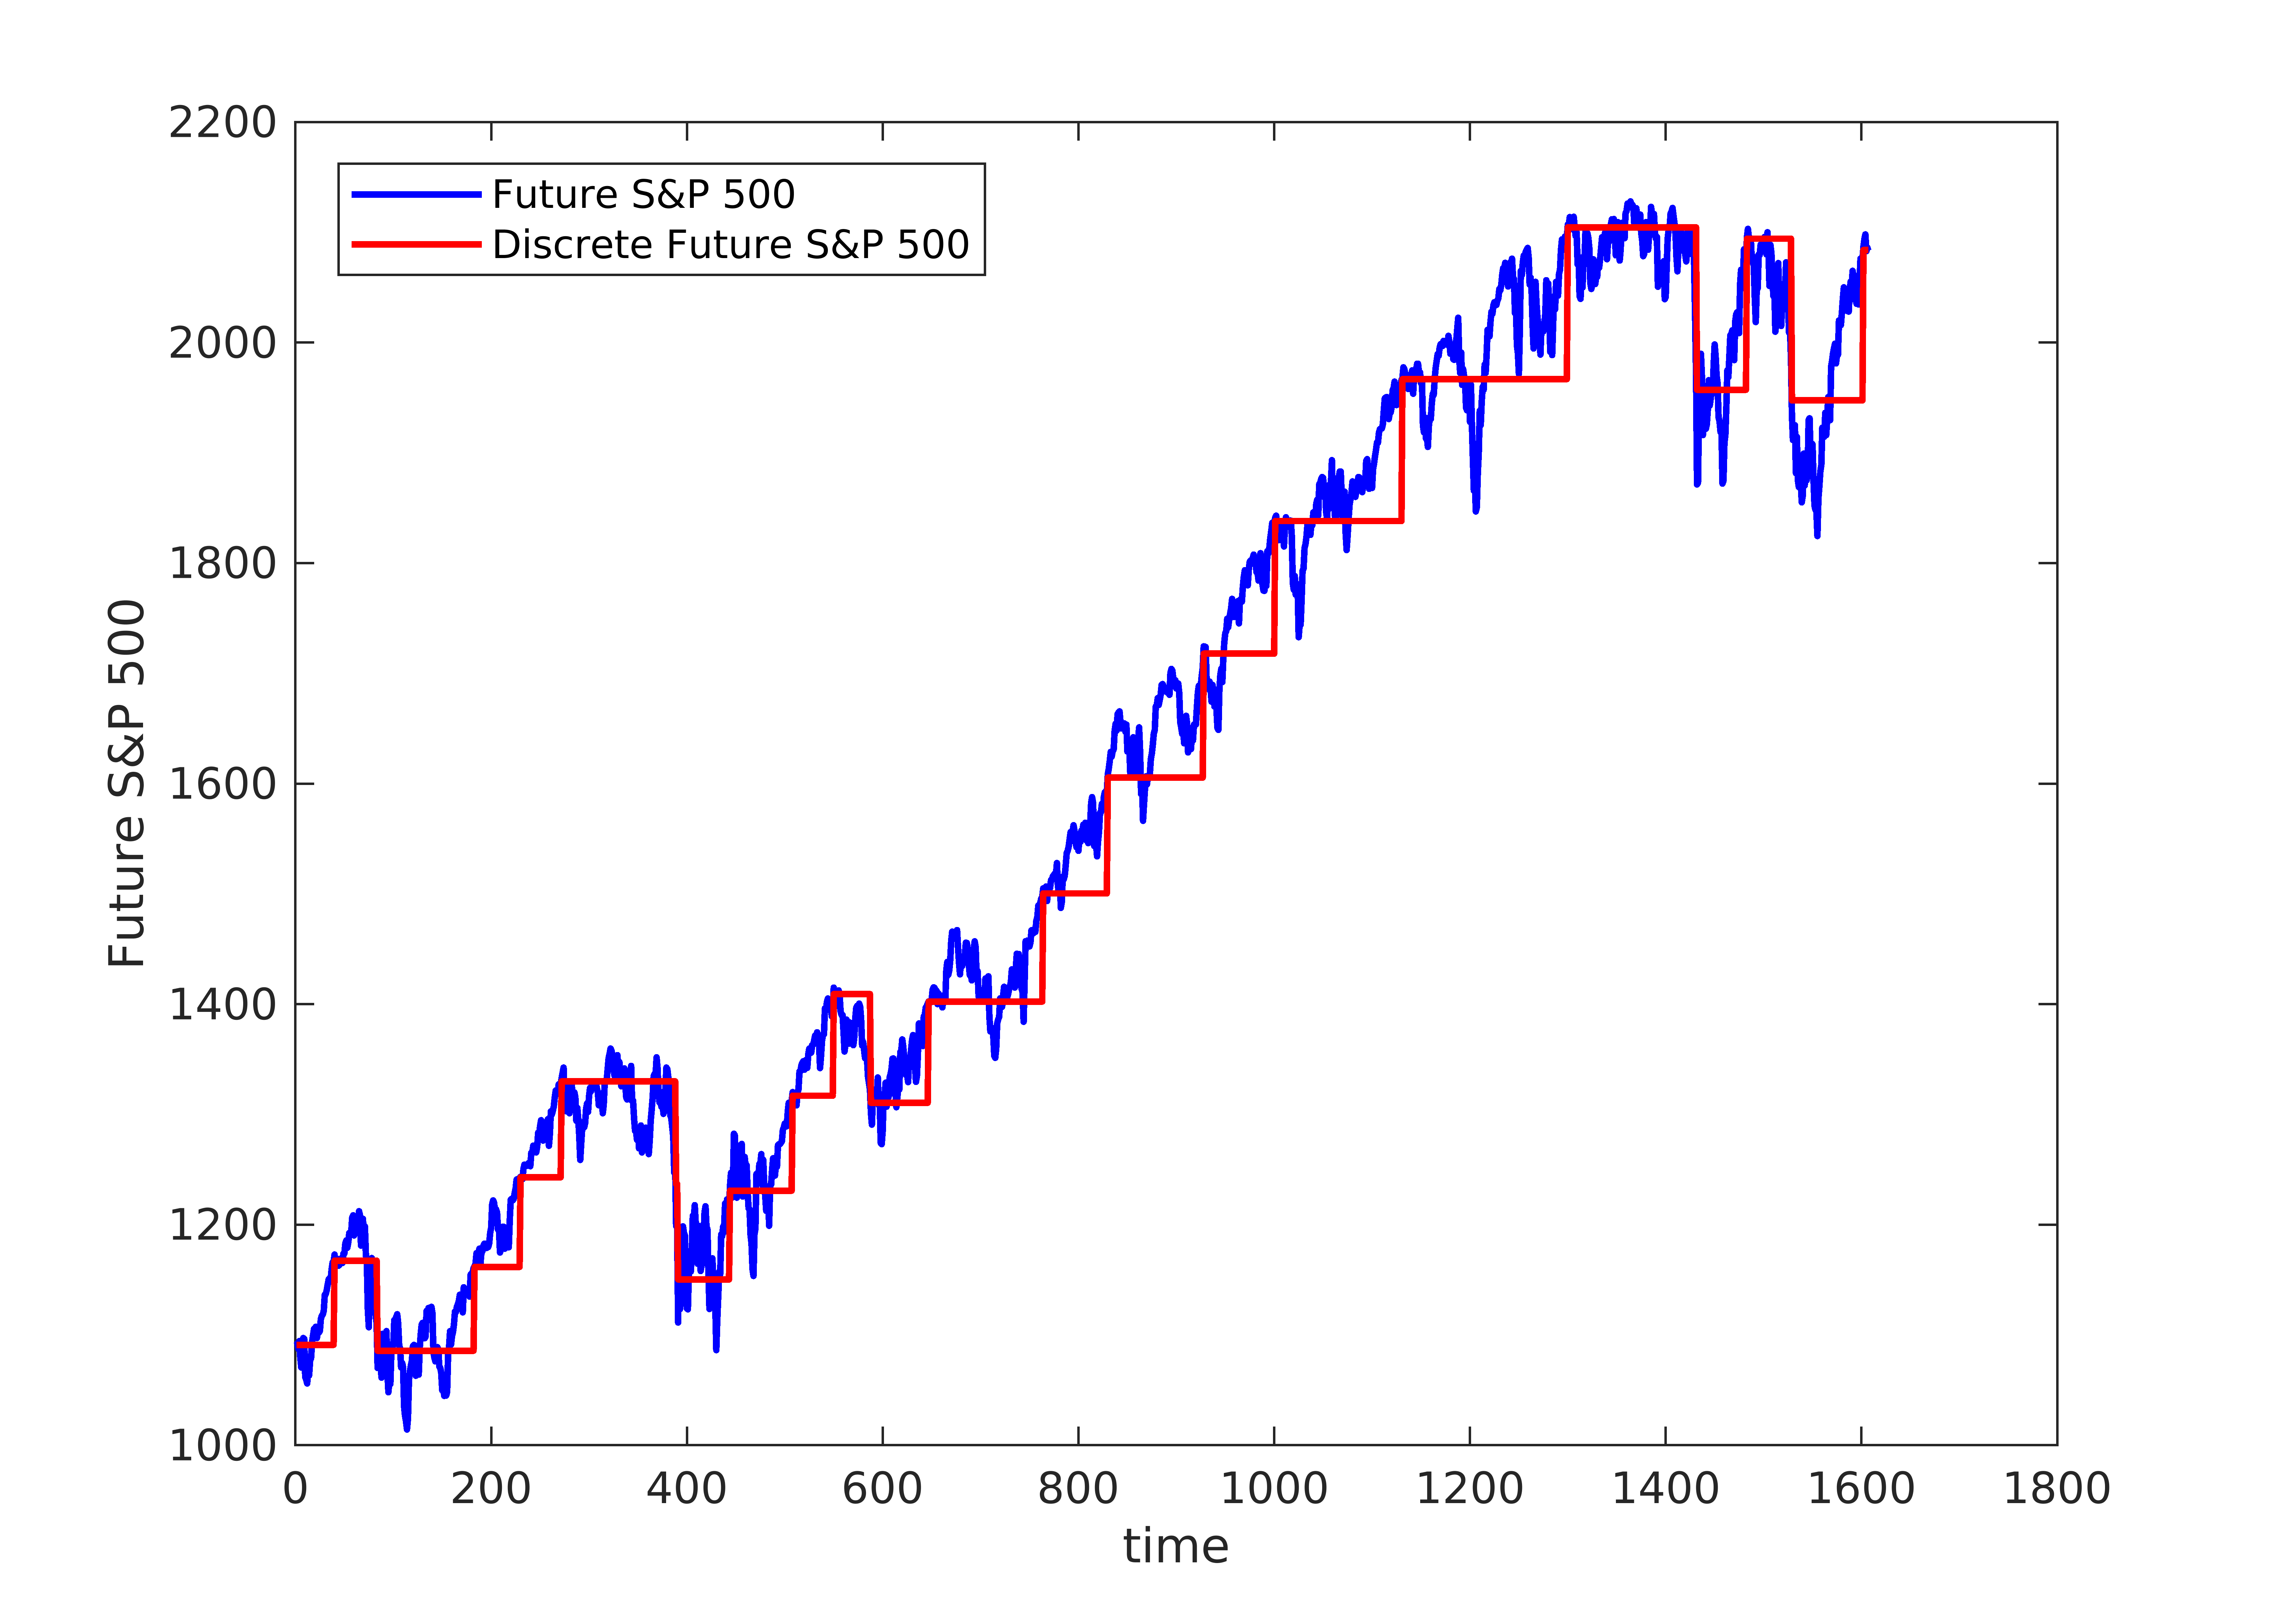
\includegraphics[scale = 0.7]{Images/DiscreteDynamics}
	\caption{Future S\&P 500 and its discrete time series. The discrete time series was obtained with a jump size $J=7\%$}
	\label{fig:DiscreteDynamics}
\end{figure}
The likelihood function can be written as follows
\begin{equation*}
\begin{split}
L(\lambda,p;\mathbf{y}) & = \prod_{i=1}^{n}f_{N^{\Delta t}_{k+1}}(y_i;\lambda,p)\\
& =\Big(\prod_{y_i = 0}\exp(-\lambda\Delta t) \Big)
\Big(\prod_{y_i=1}\big(1-\exp(-\lambda\Delta t) \big)p \Big)
\Big(\prod_{y_i=-1}\big(1-\exp(-\lambda\Delta t)\big)(1-p) \Big)\\
& = \Big(\exp(-\lambda\Delta t) \Big)^\alpha
\Big(\big(1-\exp(-\lambda\Delta t) \big)p \Big)^\beta
\Big(\big(1-\exp(-\lambda\Delta t)\big)(1-p) \Big)^\gamma
\end{split}
\end{equation*}
where 
con 
\[ \alpha =  \text{card}\{y_i = 0 \colon i = 1,\ldots,n\}\]
\[ \beta =  \text{card}\{y_i = 1 \colon i = 1,\ldots,n\}\]
\[ \gamma =  \text{card}\{y_i = -1 \colon i = 1,\ldots,n\}\]
and $\Delta t$ has been set to 1/252. Imposing the first order optimality condition $\nabla \log(L(\lambda,p;\mathbf{y}))=\bm{0}$
and solving with respect to $p$ and $\lambda$ we obtain the following estimates
\begin{align}
\widehat{\lambda} &= -\frac{1}{\Delta t}\log\Big(\frac{\alpha}{\alpha+\beta+\gamma}\Big)\\[2ex]
\widehat{p}& = \frac{\beta}{\beta+\gamma}
\end{align}
The point $(\widehat{p},\widehat{\lambda})$ is actually a maximizer since the Hessian matrix computed in this point is definite negative.
\begin{remark}
	As $\alpha+\beta+\gamma$ equals $n$ (the sample size), the estimator of $\lambda$ depends only on the number of interval in which there are no jumps ($\alpha$). Conversely, the estimator of $p$ depends only on the number of positive and negative jumps, as it was reasonable to expect.  
\end{remark}
\section{Numerical Results}
\begin{figure}
	%\centering
	\makebox[\textwidth][c]{
	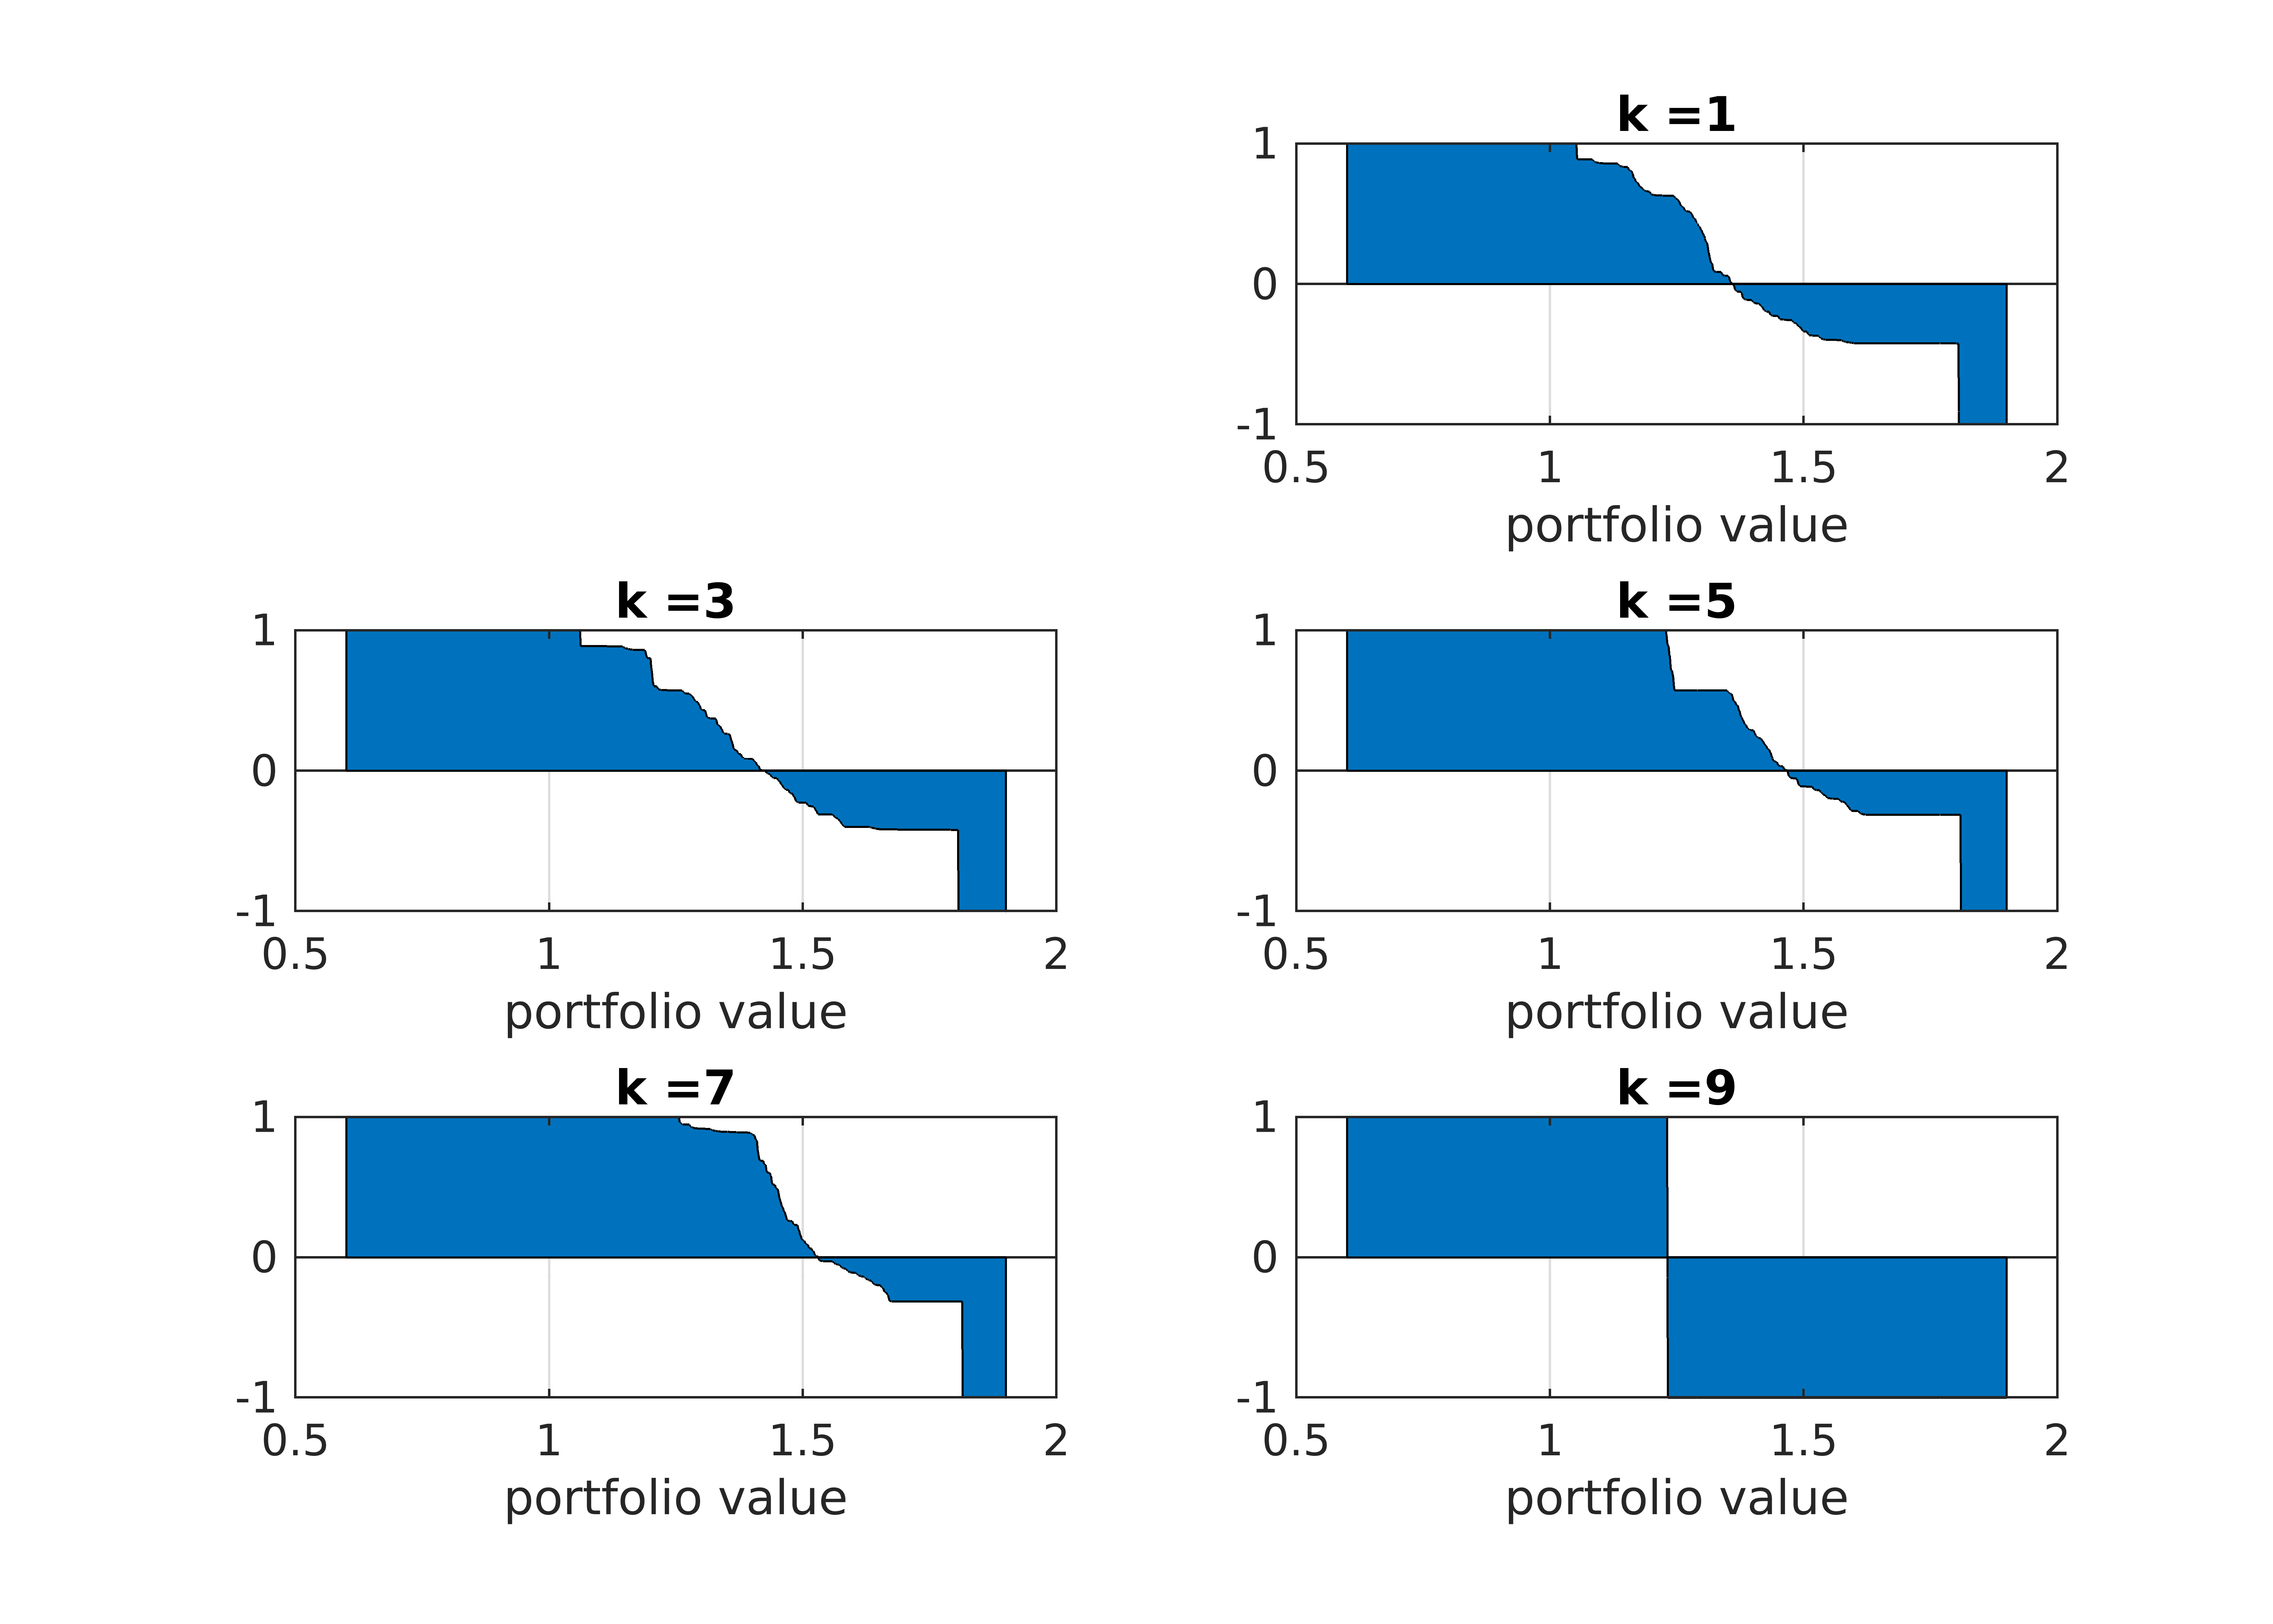
\includegraphics[scale = 0.6]{Images/mapsbasic}}
	\caption{allocation maps}
	\label{fig:basic_maps}
\end{figure}


